\section{Analytical Model}
\label{sec:analytical-model}
In this Section we define the analytical model of the system.
%
In particular, we will show the queue model, Markov Chain and performance metrics formulas for the system both running the Off-Loading Policy 1 and the Off-Loading Policy 2.
%
At the end, we will explain how we solved the analytical model to obtain theoretical results for the target case.

\paragraph{Queue Model}
As the system is characterized by Poisson arrivals and Exponential services, we could consider treating the queue model as a Jackson Network. 
Nevertheless, this would not be correct without a very strong assumption on the routing probabilities, In fact, a Jackson Network requires the routing probabilities  to be static, i.e. independent of the system state, and this is not the case.

So, \textit{we assume the routing probabilities to be static in order to unlock the potential of the Jackson Network in our analytical dissertation}.

In Figures~\ref{fig:analytical-model-queue-1} and \ref{fig:analytical-model-queue-2}, we show the queue models for the system with Off-Loading Policy 1 and Off-Loading Policy 2, respectively.

\begin{figure}delphi
	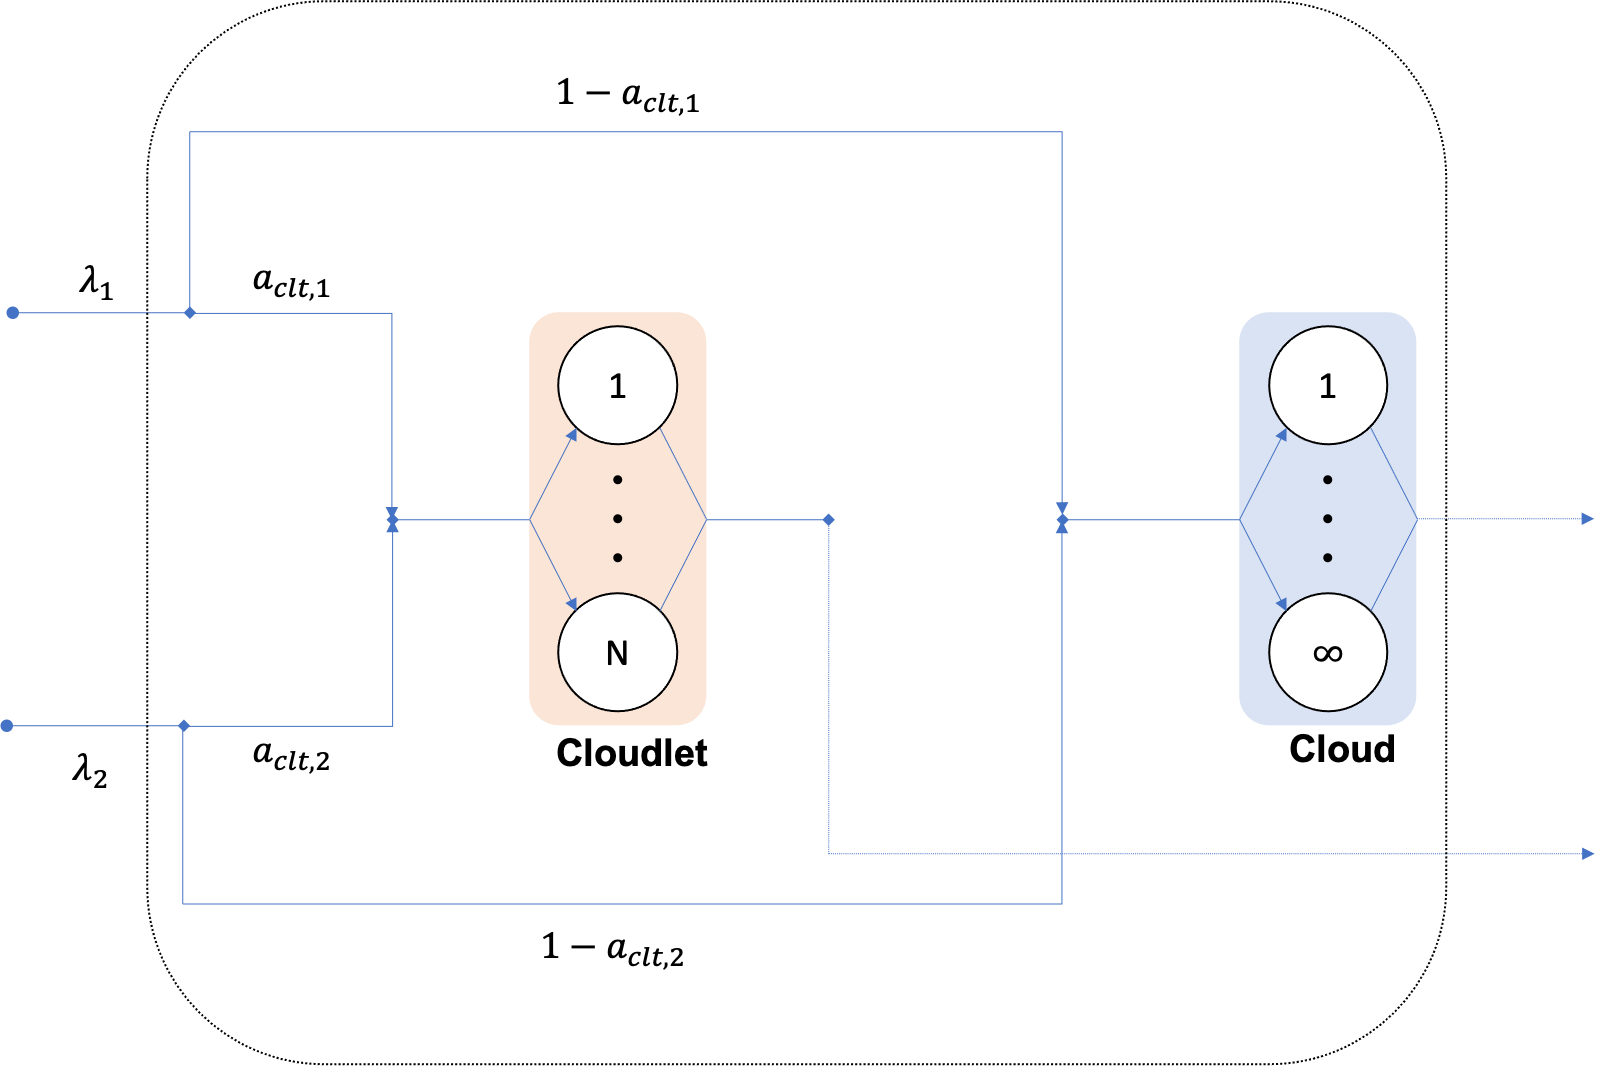
\includegraphics[width=\columnwidth]{fig/analytical-model-queue-1}
	\caption{Queue model for the system with OP1.}
	\label{fig:analytical-model-queue-1}
\end{figure}

\begin{figure}
	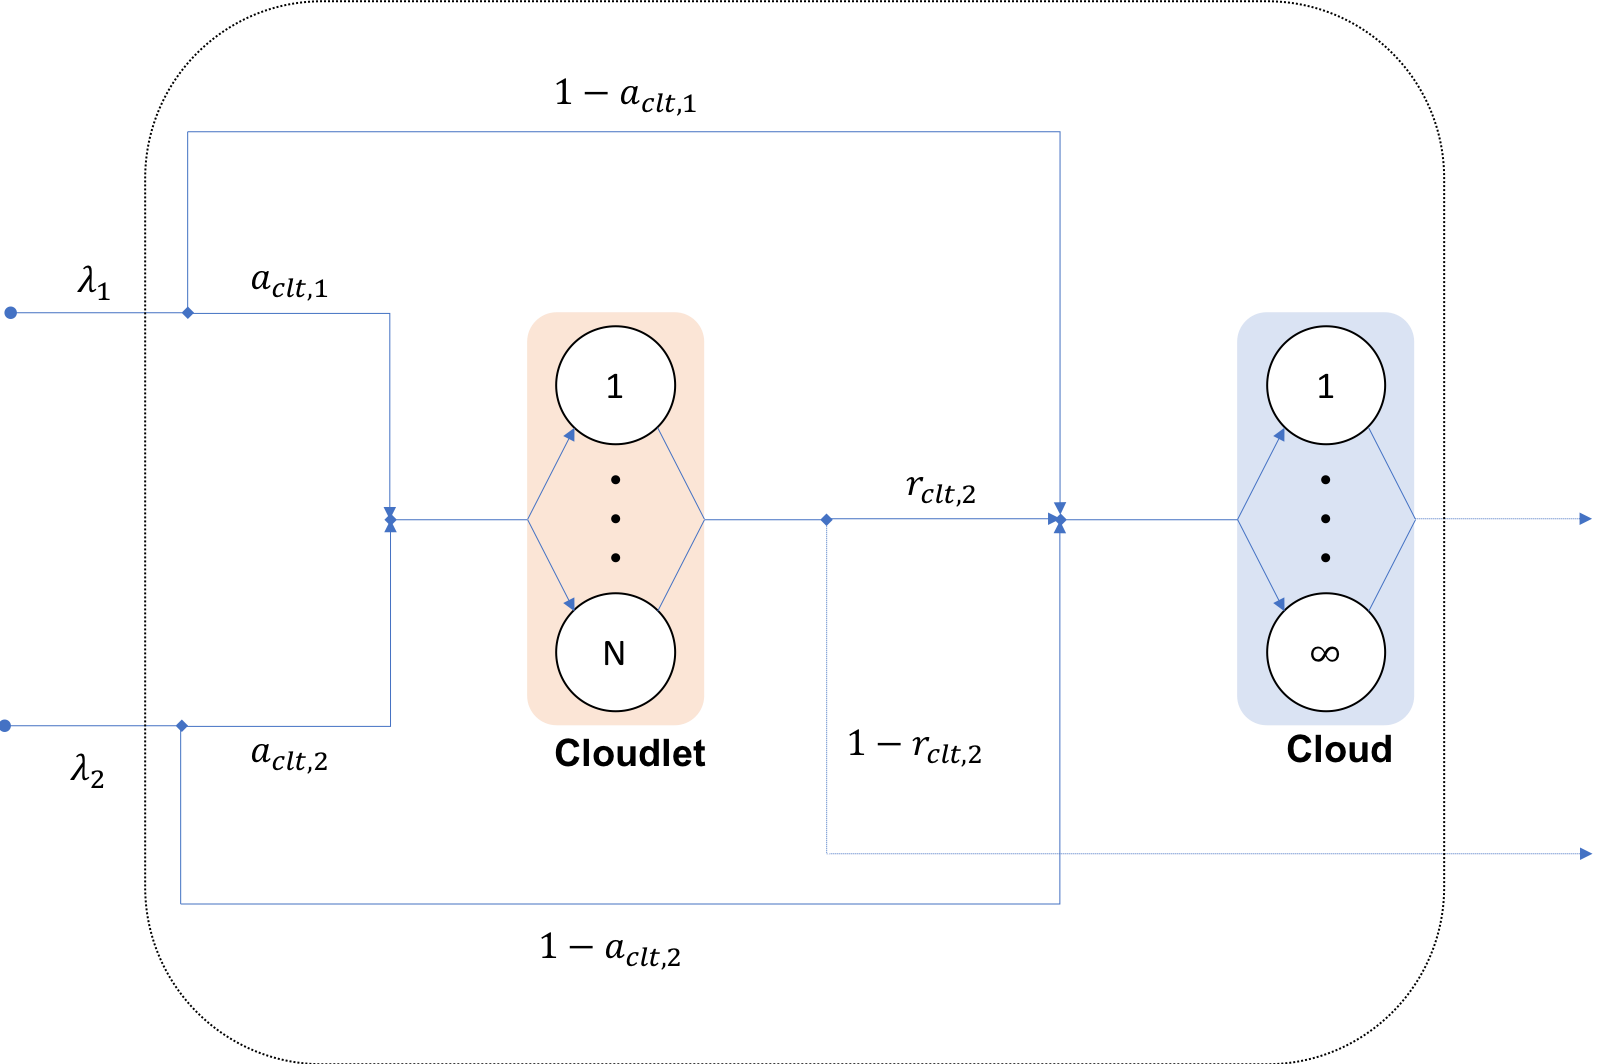
\includegraphics[width=\columnwidth]{fig/analytical-model-queue-2}
	\caption{Queue model for the system with OP2.}
	\label{fig:analytical-model-queue-2}
\end{figure}

The definition of the routing probabilities relies on the following subsets of Cloudlet states $S_{clt}$, whose definition strictly depends on the adopted off-loading policy:

\begin{itemize}
	\item $A_{clt,1}$:  subset of states where a task belonging to the $1^{st}$ class is accepted in the Cloudlet.
	
	In OP1, a $1^{st}$ class task is accepted in the Cloudlet as long as not all the $N$ resources are occupied.
	In OP2, a $1^{st}$ class task is accepted in the Cloudlet as long as not all the $N$ resources are occupied or there is at least one $2^{nd}$ class task to be interrupted.

	\begin{equation}
		A_{clt,1} :=
		\left\{
		\begin{array}{ll}
			\begin{aligned}
				& \{(n_{clt,1},n_{clt,2})\in S_{clt} : \\
				& n_{clt,1}+n_{clt,2}<N\}
			\end{aligned} & \mbox{if } OP1 \\
			\\
			\begin{aligned}
				& \{(n_{clt,1},n_{clt,2})\in S_{clt} : \\
				& n_{clt,1}+n_{clt,2}<N \vee n_{clt,2}>0\}
			\end{aligned} & \mbox{if } OP2
		\end{array}
		\right.
	\end{equation}
	
	\item $A_{clt,2}$: subset of states where  a task belonging to the $2^{nd}$ class is accepted in the Cloudlet.
	
	In OP1, a $2^{nd}$ class task is accepted in the Cloudlet as long as not all the $N$ resources are occupied.
	In OP2, a $2^{nd}$ class task is accepted in the Cloudlet as long as not all the $N$ resources are occupied and there are at most $S$ resources occupied by $2^{nd}$ class tasks.
	
	\begin{equation}
		A_{clt,2} :=
		\left\{
		\begin{array}{ll}
			\begin{aligned}
				& \{(n_{clt,1},n_{clt,2})\in S_{clt} : \\
				& n_{clt,1}+n_{clt,2}<N\}
			\end{aligned} & \mbox{if } OP1 \\
			\\
			\begin{aligned}
				& \{(n_{clt,1},n_{clt,2})\in S_{clt} : \\
				& n_{clt,1}+n_{clt,2}<N \wedge n_{clt,2}<S\}
			\end{aligned} & \mbox{if } OP2
		\end{array}
		\right.
	\end{equation}
	
	\item $R_{clt,2}$: subset of states where  a task belonging to the $2^{nd}$ class is interrupted in the Cloudlet and it is restarted in the Cloud.
	
	In OP1, the set is empty because task interruption is not provided by the policy.
	In OP2, a $2^{nd}$ class task is interrupted in the Cloudlet and restarted in the Cloud as long as the former does not have free resources and there is at least one $2^{nd}$ class task to interrupt.
	
	\begin{equation}
		R_{clt,2} :=
		\left\{
		\begin{array}{ll}
			\begin{aligned}
				& \emptyset
			\end{aligned} & \mbox{if } OP1 \\
			\\
			\begin{aligned}
				& \{(n_{clt,1},n_{clt,2})\in S_{clt} : \\
				& n_{clt,1}+n_{clt,2}=N \wedge n_{clt,2}>0\}
			\end{aligned} & \mbox{if } OP2
		\end{array}
		\right.
	\end{equation}
\end{itemize}

Given such sets, the routing probabilities  are accordingly defined:

\begin{itemize}
	
	\item $a_{clt,1}$: the probability for a demanding $1^{st}$ class task to be accepted in the Cloudlet.
	
	\begin{equation} 
		a_{clt,1} := \sum_{s\in A_{clt,1}} \pi_{s}
	\end{equation}
	
	\item $a_{clt,2}$: the probability for a demanding $2^{nd}$ class task to be accepted in the Cloudlet.
	
	\begin{equation} 
		a_{clt,2} := \sum_{s\in A_{clt,2}} \pi_{s}
	\end{equation}
		
	\item $r_{clt,2}$: the probability for a running $2^{nd}$ class task to be interrupted in the Cloudlet and restarted in the Cloud.
	
	\begin{equation} 
		\begin{split}
			r_{clt,2} & = \sum_{s\in R_{clt,2}} \pi_{s} \Big(\frac{\lambda_{1}}{\lambda_{1}+\lambda_{2}}\Big) \\
		\end{split}
	\end{equation}
\end{itemize}

\paragraph{Markov Chain}
As the system is characterized by Poisson arrivals\footnote{same as Exponential inter-arrivals.} and Exponential services, the Markovian condition holds true and we can then determine the Markov Chain\footnote{If the Markovian condition is not satisfied, Markov Chain solution must be considered only as an approximation.} whose resolution allows us to compute the routing probabilities.

For sake of simplicity, we consider here the simple case with $N=2$ in order to (i) give an idea of the system of equations to be solved and (ii) graphically recognize the critical states. 
In fact, the representation fo the Markov Chain and the associated equations would be impractical for the target case $N=20$, due to the combinatorial explosion of the state space.

In Figure~\ref{fig:analytical-model-markov-1} we show the Markov Chain for the system with Off-Loading Policy 1 and $N=2$. 
In this chain, red states represent those where both the $1^{st}$ and $2^{nd}$ class traffic is blocked by the Cloudlet and forwarded to the Cloud.
The associated flow balance equations are listed in Equation~\ref{eqn:analytical-model-markov-1}.

\begin{figure}
	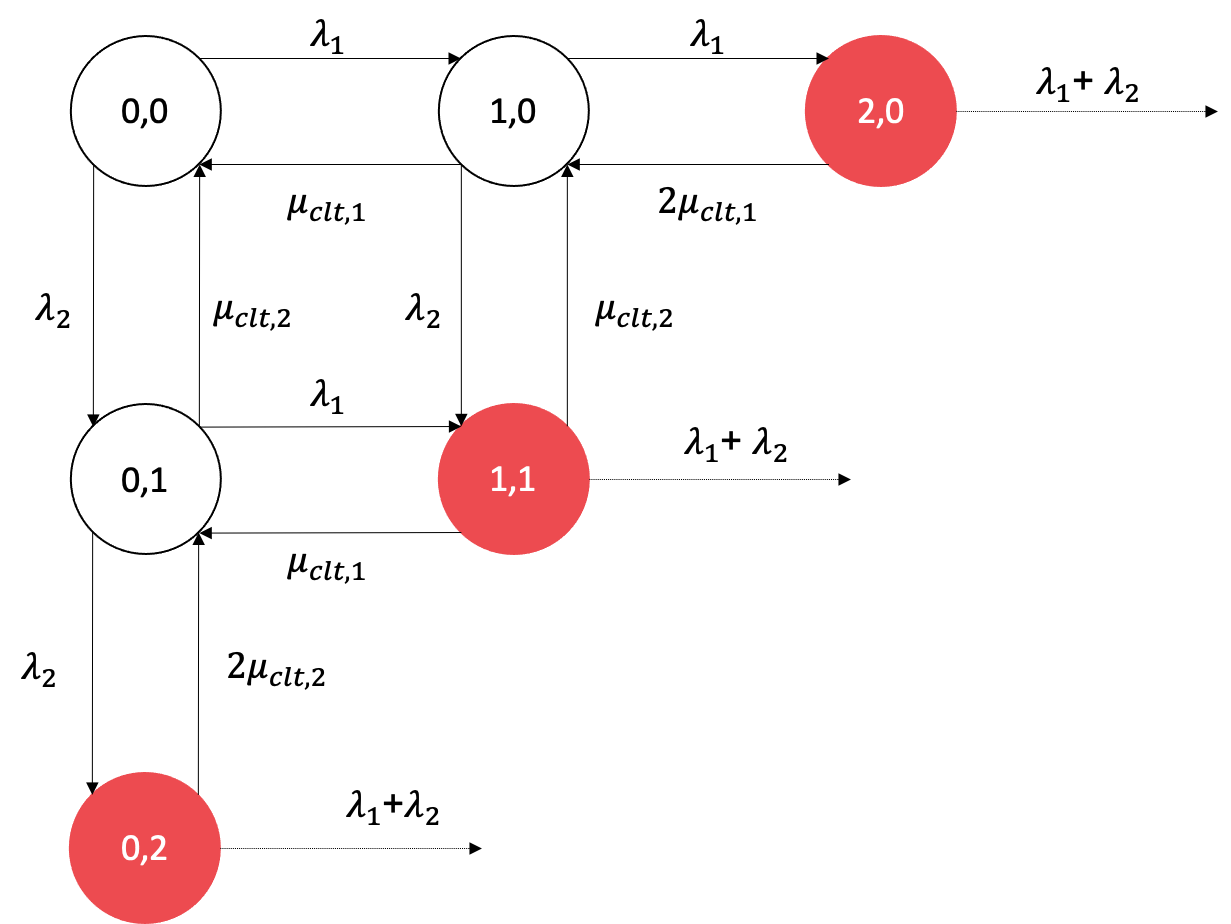
\includegraphics[width=\columnwidth]{fig/analytical-model-markov-1}
	\caption{Markov Chain for the system with OP1 (N=2).}
	\label{fig:analytical-model-markov-1}
\end{figure}

\begin{equation}
	\begin{split}
		\pi_{0,0}(\lambda_{1}+\lambda_{2})& = \pi_{1,0}\mu_{clt,1}+\pi_{0,1}\mu_{clt,2} \\
		\pi_{0,1}(\lambda_{1}+\lambda_{2}+\mu_{clt,2}) & = \pi_{0,0}\lambda_{2}+\pi_{1,1}\mu_{clt,1}+\pi_{0,2}2\mu_{clt,2} \\
		\pi_{1,0}(\lambda_{1}+\lambda_{2}+\mu_{clt,1}) & = \pi_{0,0}\lambda_{1}+\pi_{1,1}\mu_{clt,2}+\pi_{2,0}2\mu_{clt,1} \\
		\pi_{1,1}(\mu_{clt,1}+\mu_{clt,2}) & = \pi_{0,1}\lambda_{1}+\pi_{1,0}\lambda_{2} \\
		\pi_{0,2}(2\mu_{clt,2}) & = \pi_{0,1}\lambda_{2} \\
		\pi_{2,0}(2\mu_{clt,1}) & = \pi_{1,0}\lambda_{1} \\
		1 & = \pi_{0,0}+\pi_{0,1}+\pi_{1,0}+\pi_{1,1}+\pi_{0,2}+\pi_{2,0}\\
	\end{split}
	\label{eqn:analytical-model-markov-1}
\end{equation}

In Figure~\ref{fig:analytical-model-markov-2} we show the Markov Chain for the system with Off-Loading Policy 2 and $N=S=2$. 
In this chain, the red state represents the one where both the $1^{st}$ and $2^{nd}$ class traffic is blocked; whereas the orange states represent those where (i) a $1^{st}$ class arrival is accepted in Cloudlet, causing the restart in Cloud of a random running $2^{nd}$ class task and (ii) a $2^{nd}$ class arrival is blocked by the Cloudlet and forwarded to the Cloud.

\begin{figure}
	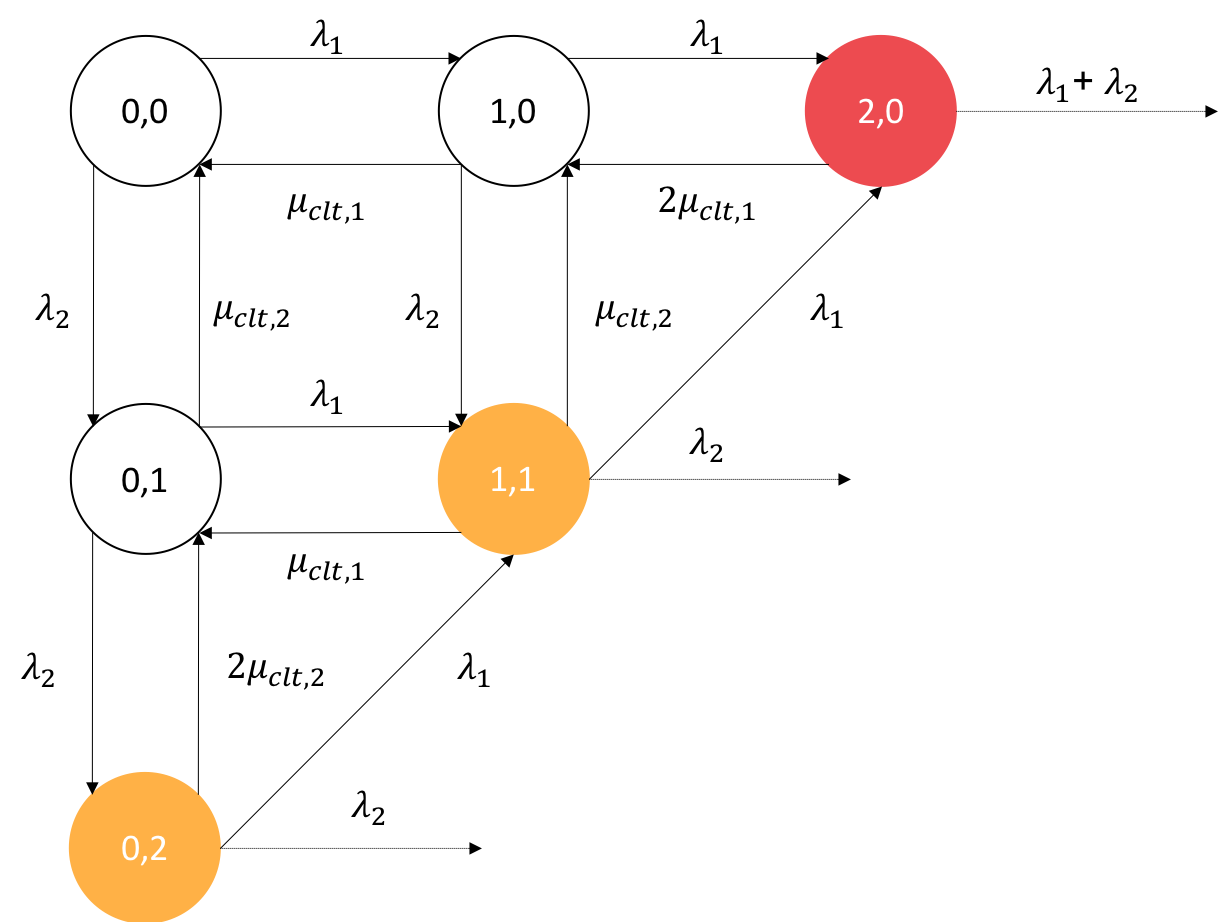
\includegraphics[width=\columnwidth]{fig/analytical-model-markov-2}
	\caption{Markov Chain for the system with OP2 (N=S=2).}
	\label{fig:analytical-model-markov-2}
\end{figure}

\begin{equation}
	\begin{split}
		\pi_{0,0}(\lambda_{1}+\lambda_{2})& = \pi_{1,0}\mu_{clt,1}+\pi_{0,1}\mu_{clt,2} \\
		\pi_{0,1}(\lambda_{1}+\lambda_{2}+\mu_{clt,2}) & = \pi_{0,0}\lambda_{2}+\pi_{1,1}\mu_{clt,1}+\pi_{0,2}2\mu_{clt,2} \\
		\pi_{1,0}(\lambda_{1}+\lambda_{2}+\mu_{clt,1}) & = \pi_{0,0}\lambda_{1}+\pi_{1,1}\mu_{clt,2}+\pi_{2,0}2\mu_{clt,1} \\
		\pi_{1,1}(\lambda_{1}+\mu_{clt,1}+\mu_{clt,2}) & = \pi_{0,1}\lambda_{1}+\pi_{1,0}\lambda_{2}+\pi_{0,2}\lambda_{1} \\
		\pi_{0,2}(\lambda_{1}+2\mu_{clt,2}) & = \pi_{0,1}\lambda_{2} \\
		\pi_{2,0}2\mu_{clt,1} & = \pi_{1,0}\lambda_{1}+\pi_{1,1}\lambda_{1} \\
		1 & = \pi_{0,0}+\pi_{0,1}+\pi_{1,0}+\pi_{1,1}+\pi_{0,2}+\pi_{2,0}\\
	\end{split}
	\label{eqn:analytical-model-markov-2}
\end{equation}

In Figure~\ref{fig:analytical-model-markov-2-1} we show the Markov Chain for the system with Off-Loading Policy 2 and $N=2,S=1$. 
In this chain, the red state represents the one where both the $1^{st}$ and $2^{nd}$ class traffic is blocked; the orange state represents the one where (i) a $1^{st}$ class arrival is accepted in Cloudlet, causing the restart in Cloud of a random running $2^{nd}$ class task and (ii) a $2^{nd}$ class arrival is blocked by the Cloudlet and forwarded to the Cloud; whereas the grey state and (ii) a $2^{nd}$ class arrival is blocked by the Cloudlet and forwarded to the Cloud.

\begin{figure}
	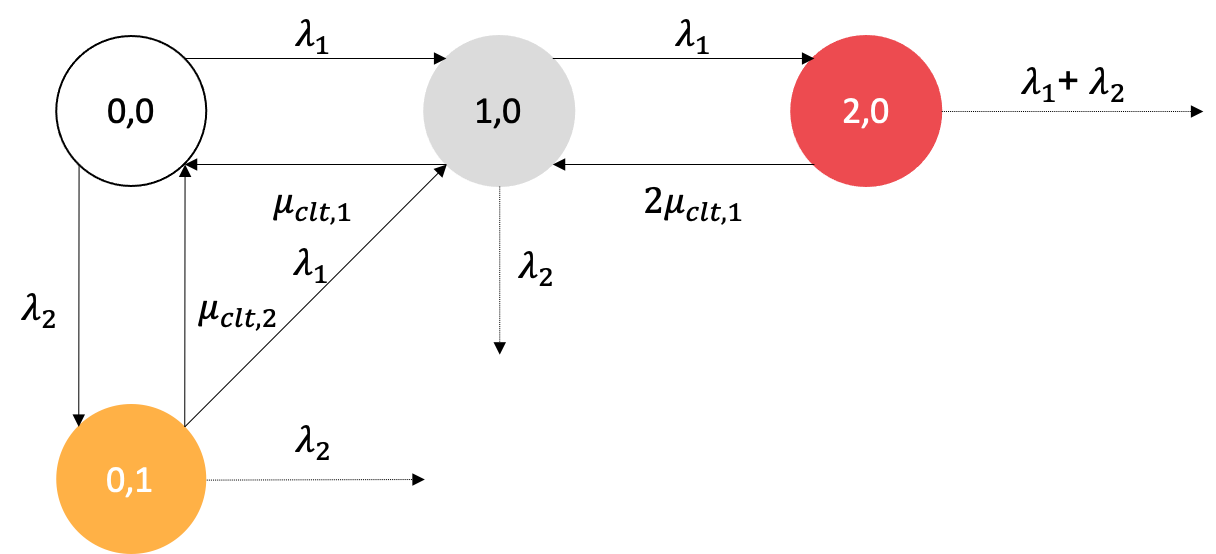
\includegraphics[width=\columnwidth]{fig/analytical-model-markov-2-1}
	\caption{Markov Chain for the system with OP2 (N=2, S=1).}
	\label{fig:analytical-model-markov-2-1}
\end{figure}

\begin{equation}
	\begin{split}
		\pi_{0,0}(\lambda_{1}+\lambda_{2})& = \pi_{1,0}\mu_{clt,1}+\pi_{0,1}\mu_{clt,2} \\
		\pi_{0,1}(\lambda_{1}+\mu_{clt,2}) & = \pi_{0,0}\lambda_{2} \\
		\pi_{1,0}(\lambda_{1}+\mu_{clt,1}) & = \pi_{0,0}\lambda_{1}+\pi_{2,0}2\mu_{clt,1} \\
		\pi_{2,0}2\mu_{clt,1} & = \pi_{1,0}\lambda_{1} \\
		1 & = \pi_{0,0}+\pi_{0,1}+\pi_{1,0}+\pi_{2,0}\\
	\end{split}
	\label{eqn:analytical-model-markov-2-1}
\end{equation}

\paragraph{Accepted Workload}
Given the routing probabilities we can determine the following accepted workloads:

\begin{itemize}
	\item \textit{Cloudlet}: arrival rate of tasks belonging to $j$-th class accepted in Cloudlet, valid both for OP1 and OP2:
	\begin{equation}
	\lambda_{clt,j} = a_{clt,j}\lambda_{j}
	\end{equation}
	
	\item \textit{Cloud}: arrival rate of tasks belonging to $j$-th class forwarded to Cloud, valid both for OP1 and OP2:
	\begin{equation}
	\lambda_{cld,j} = (1-a_{clt,j})\lambda_{j}
	\end{equation}
	
	\item \textit{Restarts}: rate of tasks belonging to $2^{nd}$ class interrupted in Cloudlet and restarted in Cloud, valid only for OP2:
	\begin{equation}
	\lambda_{r} = r(\lambda_{1}+\lambda_{2})
	\end{equation}
\end{itemize}

\paragraph{Performance metrics}
Given the accepted workloads we can determine the following performance metrics for classed tasks in each subsystem\footnote{In every formula, we omitted the symbol $E[\cdot]$ of the expected value in order to lighten the notation.}.

\begin{itemize}
	
	\item $1^{st}$ class in Cloudlet:
	\begin{equation} 
		\begin{split}
			N_{clt,1} &= \sum_{s: (n_{clt,1},n_{clt,2}) \in S_{clt}} \pi_{s} n_{clt,1}  \\
			X_{clt,1} &= \lambda_{clt,1} \\
			T_{clt,1} &= \frac{N_{clt,1}}{X_{clt,1}} \\
		\end{split}
	\end{equation}

	\item $2^{nd}$ class in Cloudlet:
%\footnote{We assume here to know the expected time lost in Cloudlet by $2^{nd}$ class tasks before their interruption, i.e. $E[T_{clt,2,lost}]$.In particular, as we are not able to determine it from the Markov Chain in a simple way, we will assume the experimental value computed by the simulator.}:
	\begin{equation} 
		\begin{split}
			N_{clt,2} &= \sum_{s: (n_{clt,1},n_{clt,2}) \in S_{clt}} \pi_{s} n_{clt,2}  \\
			%E[N_{clt,2}] &= \lambda_{clt,2}E[T_{clt,2}]-\lambda_{r} E[T_{clt,2,lost}] \\
			%E[N_{clt,2}] &= \lambda_{clt,2}E[T_{clt,2}]-E[N_{cld,2}]^{[R]} \\
			X_{clt,2} &= \lambda_{clt,2} - \lambda_{r} \\
			T_{clt,2} &= \frac{N_{clt,2}}{X_{clt,2}} \\
		\end{split}
	\end{equation}

It is important to notice here that we assumed that the Cloudlet throughput for $2^{nd}$ class tasks is only given by the portion of traffic that is served to completion by the Cloudlet, thus excluding the portion of interrupted traffic.

	\item $1^{st}$ class in Cloud:
	\begin{equation} 
		\begin{split}
			T_{cld,1} &= \frac{1}{\mu_{cld,1}} \\
			N_{cld,1} &= \lambda_{cld,1}T_{cld,1} \\
			X_{cld,1} &= \lambda_{cld,1} \\
		\end{split}
	\end{equation}
	
	\item $2^{nd}$ class in Cloud (NR: not restarted\footnote{$2^{nd}$ class tasks that are served by the Cloud because they have not been accepted in the Cloudlet.}):
	\begin{equation} 
	\begin{split}
		T_{cld,2}^{[NR]} &= \frac{1}{\mu_{cld,2}} \\
		N_{cld,2}^{[NR]} &= \lambda_{cld,2}T_{cld,2}^{[NR]} \\
		X_{cld,2}^{[NR]} &= \lambda_{cld,2} \\
	\end{split}
	\end{equation}
	
	\item $2^{nd}$ class in Cloud (R: restarted\footnote{$2^{nd}$ class tasks that are served by the Cloud because they have been interrupted in the Cloudlet.}):
	\begin{equation} 
	\begin{split}
		T_{cld,2}^{[R]} &= T_{setup}+ T_{cld,2}^{[NR]} \\
		N_{cld,2}^{[R]} &= \lambda_{r} T_{cld,2}^{[R]} \\
		X_{cld,2}^{[R]} &= \lambda_{r} \\
	\end{split}
	\end{equation}

	It is important to notice here that we decided to assign the entire setup time to the Cloud.
	
	\item $2^{nd}$ class in Cloud (both restarted and not restarted):
	\begin{equation} 
	\begin{split}
		T_{cld,2} &= \sum_{m=NR,R} \frac{N_{cld,2}^{[m]}}{N_{cld,2}}T_{cld,2}^{[m]} \\
		N_{cld,2} &= \sum_{m=NR,R} N_{cld,2}^{[m]} \\
		X_{cld,2} &= \sum_{m=NR,R} X_{cld,2}^{[m]} \\
	\end{split}
	\end{equation}
\end{itemize}

Then we can determine the following performance metrics for each subsystem:

\begin{itemize}
	\item Cloudlet:
	\begin{equation} 
	\begin{split}
		T_{clt} &= \sum_{j=1,2} \frac{N_{clt,j}} {N_{clt}} T_{clt,j} \\
		N_{clt} &= \sum_{j=1,2} N_{clt,j} \\
		X_{clt} &= \sum_{j=1,2} X_{clt,j} \\
	\end{split}
	\end{equation}
	
	\item Cloud:
	\begin{equation} 
	\begin{split}
		T_{cld} &= \sum_{j=1,2} \frac{N_{cld,j}} {N_{cld}} T_{cld,j} \\
		N_{cld} &= \sum_{j=1,2} N_{cld,j} \\
		X_{cld} &= \sum_{j=1,2} X_{cld,j} \\
	\end{split}
	\end{equation}

	It is important to notice here that we assumed that the Cloud throughput is given by all the traffic that is served to completion by the Cloudlet, i.e. both the portion of traffic directly assigned to the Cloud and the one that is restarted in the Cloud.
	\end{itemize}

Finally, we can determine the following performance metrics for the whole system:

\begin{equation} 
\begin{split}
	T &= \sum_{i=cld,clt} \frac{N_{i}} {N} T_{i} \\
	N &= \sum_{i=cld,clt} N_{i} \\
	X &= \sum_{i=cld,clt} X_{i} \\
\end{split}
\end{equation}


\paragraph{Resolution}
We solved the analytical models with a custom Python script executing the following steps:

\begin{itemize}
\item receives as input the system configuration
\item  generates the Markov Chain representing the Cloudlet
\item  generates the system of equations from the Markov Chain
\item  computes limiting probabilities by solving the system
\item  computes routing probabilities
\item  computes performance metrics and
\item  displays a report of results.
\end{itemize} 


Analytical results are presented in Tables~\ref{tbl:evaluation-performance-metrics-1}, \ref{tbl:evaluation-performance-metrics-2-5} and \ref{tbl:evaluation-performance-metrics-2-20}, alongside with their experimental counterparts.
%
We preferred to present analytical and experimental results in a unique common view, in order to provide the reader with an idea on how the simulator approximates analytical results.